% vim: set foldmethod=marker foldlevel=0:

\documentclass[a4paper]{article}
\usepackage[UKenglish]{babel}

\usepackage{preamble}

\usepackage{graphicx}
\graphicspath{ {./imgs/} }

\fancyhead[L]{MA150 Assignment 1}
\title{MA150 Algebra 2, Assignment 1}
\colorlet{questionbodycolor}{magenta!50}

\begin{document}

\maketitle

\setlength{\parindent}{0em}
\setlength{\parskip}{1em}

% {{{ Q1
\question{1}

\begin{questionbody}
By any means you like, solve the following system of simultaneous linear equations
\begin{align*}
2x - 5y &= b_1 \\
x - 3y &= b_2
\end{align*}
in each of the following three cases.
\end{questionbody}

\subsection{$b_1 = 0,\, b_2 = 0$} % 1.a

\begin{align*}
2x - 5y &= 0 \tag{1} \\
x - 3y &= 0 \tag{2}
\end{align*}
If a solution exists, equation $(2)$ implies $x = 3y$. Plugging this into $(1)$ gives $6x - 5y = 0$, so $y=0$. Plugging this into either equation gives $x=0$.
So if a solution exists, it must be $x=0,\, y=0$. Indeed, this solution satisfies both simultaneous equations.

\subsection{$b_1 = -3,\, b_2 = -2$} % 1.b

\begin{align*}
2x - 5y &= -3 \tag{1} \\
x - 3y &= -2 \tag{2}
\end{align*}
If a solution exists, $(1) - 2 \times (2)$ implies $0x + y = 1$, so $y=1$. Plugging this into either equation gives $x=1$.
So if a solution exists, it must be $x=1,\, y=1$. Indeed, this solution satisfies both simultaneous equations.

\begin{questionbody}
For your solution to \textbf{(b)}, sketch (reasonably accurately) the lines $2x - 5y = -3$ and
$x - 3y = -2$ in the plane $\R^2$ (labelled so as to be instantly unambiguous) and confirm
that your solution is the point where they intersect.
\end{questionbody}

\begin{center}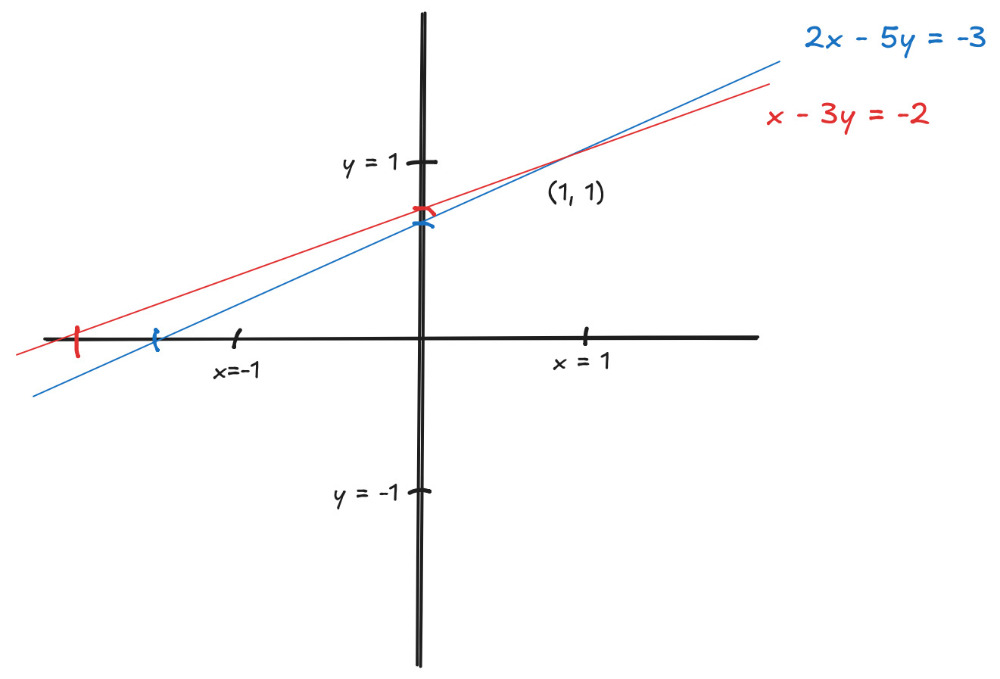
\includegraphics[scale=0.35]{Q1b}\end{center}

\subsection{$b_1 = \lambda,\, b_2 = \mu \qquad \lambda, \mu \in \R$} % 1.c

\begin{align*}
2x - 5y &= \lambda \tag{1} \\
x - 3y &= \mu \tag{2}
\end{align*}

If a solution exists, $(1) - 2 \times (2)$ implies $0x + y = \lambda - 2\mu$, so $y=\lambda - 2\mu$. Plugging this into $(2)$ gives $x = \mu + 3(\lambda - 2\mu) = 3\lambda - 5\mu$.
So if a solution exists, it must be $x=3\lambda - 5\mu,\, y=\lambda - 2\mu$. Indeed, this solution satisfies both simultaneous equations:
\begin{align*}
2(3\lambda - 5\mu) - 5(\lambda - 2\mu) = 6\lambda - 10\mu - 5\lambda + 10\mu &= \lambda \\
(3\lambda - 5\mu) - 3(\lambda - 2\mu) = 3\lambda - 5\mu - 3\lambda + 6\mu &= \mu
\end{align*}
% }}}

% {{{ Q2
\newquestion{2}

\begin{questionbody}
Solve the following linear equations
\begin{align*}
x + y + z &= b_1 \\
x - 2y + 3z &= b_2
\end{align*}
in each of the following cases.

In each case there will be infinitely many solutions, with 1 degree of freedom, and
you should find \textbf{all} solutions.
\end{questionbody}

\subsection{$b_1 = 0,\, b_2 = 0$} % 2.a

\begin{align*}
x + y + z &= 0 \tag{1} \\
x - 2y + 3z &= 0 \tag{2}
\end{align*}
The pair of simultaneous equations describes a straight line in $\R^3$. Trivially $x=0,\, y=0,\, z=0$ is a solution, so the line must pass through the origin.

To find another solution, $(1)-(2)$ implies $3y-2z=0$, so for any solution, we require $z = \f32 y$. Plugging this into either equation $(1)$ or $(2)$ gives $x + \f52 y = 0$. By observation, a solution for this is $x=5,\, y=-2$. Since $z=\f32 y$, this potential solution would also have $z=-3$. Indeed, this solution satisfies both simultaneous equations, so the line passes through $(0, 0, 0)$ and $(5, -2, -3)$.

We can parametrise the line as $\lambda \begin{pmatrix}5 \\ -2 \\ -3\end{pmatrix}$ for $\lambda \in \R$.

\subsection{$b_1 = 2,\, b_2 = 3$} % 2.b

\begin{align*}
x + y + z &= 2 \tag{1} \\
x - 2y + 3z &= 3 \tag{2}
\end{align*}
The pair of simultaneous equations describes a straight line in $\R^3$. $(1)-(2)$ implies $3y-2z=-1$, so any solution must have $z = \f32 y + \f12$. Plugging this into either equation $(1)$ or $(2)$ gives $x + \f52 y = \f32$. By observation, one solution of this equation is $x=-1,\, y=1$. This solution would require $z=2$. Indeed, this solution satisfies both simultaneous equations, so the point $(-1, 1, 2)$ is on the line.

To find more points on the line, we can rearrange the previous equation in $x$ and $y$ to get $2x+5y=3$. So when $x=0$, $y=\f35$ and this would imply $z=\f{14}{10}$. Likewise, when $y=0$, $x=\f32$ and this would imply $z=\f12$. We can check these and see that both $\l( 0, \f35, \f{14}{10} \r)$ and $\l( \f32, 0, \f12 \r)$ are on the line.

I will choose $(-1, 1, 2)$ as the fixed point for my parametrisation. The vector from $(-1, 1, 2)$ to $\l( \f32, 0, \f12 \r)$ is \[
\begin{pmatrix}\f32 \\ 0 \\ \f12\end{pmatrix}
- \begin{pmatrix}-1 \\ 1 \\ 2\end{pmatrix}
= \begin{pmatrix}\f52 \\ -1 \\ -\f32\end{pmatrix}
= \f12 \begin{pmatrix}5 \\ -2 \\ -3\end{pmatrix}
\]

Therefore we can parametrise the line as $\ds\begin{pmatrix}-1 \\ 1 \\ 2\end{pmatrix} + \lambda \begin{pmatrix}5 \\ -2 \\ -3\end{pmatrix}$ for $\lambda \in \R$.
% }}}

% {{{ Q3
\question{3}

\subsection{~} % 3.a

\begin{questionbody}
Let $\ul v = \begin{pmatrix}1 \\ 1\end{pmatrix}$ and $\ul w = \begin{pmatrix}2 \\ 1\end{pmatrix} \in \R^2$. Find the component (a real number) of $\ul v$ in the direction of $\ul w$. Compute the (vector) orthogonal projection of $\ul v$ in the direction of $\ul w$.
\end{questionbody}

The component of $\ul v$ in the direction of $\ul w$ is $\ul v \cdot \ul{\hat w}$. First, $\|\ul w\| = \sqrt5$, so $\ul{\hat w} = \df1{\sqrt5} \begin{pmatrix}2 \\ 1\end{pmatrix}$. Therefore the component of $\ul v$ in the direction of $\ul w$ is $\ds \f2{\sqrt5} + \f1{\sqrt5} = \f3{\sqrt5}$.

The orthogonal projection of $\ul v$ in the direction of $\ul w$ is \[
(\ul v \cdot \ul{\hat w})\, \ul{\hat w}
= \f3{\sqrt5}\, \f1{\sqrt5} \begin{pmatrix}2 \\ 1\end{pmatrix}
= \f35 \begin{pmatrix}2 \\ 1\end{pmatrix}
\]

\subsection{~} % 3.b

\begin{questionbody}
Let $\ul v = \begin{pmatrix}1 \\ 1 \\ 1\end{pmatrix}$ and $\ul w = \begin{pmatrix}1 \\ -2 \\ -2\end{pmatrix} \in \R^3$. Compute the orthogonal projection of $\ul v$ in the direction of $\ul w$.
\end{questionbody}

The orthogonal projection of $\ul v$ in the direction of $\ul w$ is $(\ul v \cdot \ul{\hat w})\, \ul{\hat w}$.

Firstly, $\|\ul w\| = \sqrt{1+4+4} = 3$, so $\ul{\hat w} = \df13 \begin{pmatrix}1 \\ -2 \\ -2\end{pmatrix}$. Then $\ds \ul v \cdot \ul{\hat w} = \f13 - \f23 - \f23 = -1$.

Finally, the orthogonal projection of $\ul v$ in the direction of $\ul w$ is \[
(\ul v \cdot \ul{\hat w})\, \ul{\hat w}
= - \ul{\hat w}
= \f13 \begin{pmatrix}-1 \\ 2 \\ 2\end{pmatrix}
\]
% }}}

% {{{ Q4
\newquestion{4}

\begin{questionbody}
Let $P = \begin{pmatrix}1 \\ 1 \\ 1\end{pmatrix}$ and $Q = \begin{pmatrix}1 \\ -1 \\ 3\end{pmatrix} \in \R^3$, on which we have coordinates $x, y z$.
\end{questionbody}

\subsection{~} % 4.a

\begin{questionbody}
Give the equation of the plane $\Pi \in \R^3$ that passes through $P$, $Q$, and the origin $\ul 0 \in \R^3$.
\end{questionbody}

The plane will have equation $\begin{pmatrix}x \\ y \\ z\end{pmatrix} \cdot \ul{\hat n} = 0$, where $\ul{\hat n}$ is a unit normal vector to the plane. We can find $\ul n$ with the cross product: \[
\ul n = \overrightarrow{P\;} \times \overrightarrow{Q\;}
= \begin{pmatrix}1 \\ 1 \\ 1\end{pmatrix}
\times \begin{pmatrix}1 \\ -1 \\ 3\end{pmatrix}
= \begin{pmatrix}4 \\ -2 \\ -2\end{pmatrix}
\]

Then $\|\ul n\| = \sqrt{16+4+4} = 2\sqrt6$, so $\ul{\hat n} = \df1{2\sqrt6} \begin{pmatrix}4 \\ -2 \\ -2\end{pmatrix} = \df1{\sqrt6} \begin{pmatrix}2 \\ -1 \\ -1\end{pmatrix}$

Therefore $\Pi$ has equation $\f1{\sqrt6} \l( 2x - y - z \r) = 0$. Or equivalently, $2x - y - z = 0$.

\subsection{~} % 4.b

\begin{questionbody}
Give two equations that together define the line $L_{PQ}$ through $P$ and $Q$.
\end{questionbody}

We need two equations that define planes containing $P$ and $Q$. We've already got the plane through the origin.

The point $(1, 0, 0)$ does not satisfy the equation of the plane from part \textbf{(a)}, so it is not on the plane $\Pi$. It also therefore not collinear with $P$ and $Q$, so we can use it to find a different plane, $\Pi_2$.

For this plane, we need the normal vector from before, which we find slightly differently, since $\Pi_2$ doesn't include the origin, so we can't just use the position vectors of $P$ and $Q$. Let's call $(1, 0, 0)$ the point $X$.

\begin{align*}
\ul n &= \overrightarrow{XP\;} \times \overrightarrow{XQ\;} \\[1ex]
&= \l(\overrightarrow{P\;} - \overrightarrow{X\;}\r) \times \l(\overrightarrow{Q\;} - \overrightarrow{X\;}\r) \\[1ex]
&= \begin{pmatrix}0 \\ 1 \\ 1\end{pmatrix} \times \begin{pmatrix}0 \\ -1 \\ 3\end{pmatrix} \\[1ex]
&= \begin{pmatrix}4 \\ 0 \\ 0\end{pmatrix} \\[1ex]
\thf \ul{\hat n} &= \begin{pmatrix}1 \\ 0 \\ 0\end{pmatrix}
\end{align*}

Then $\Pi_2$ is defined by $x + 0y + 0z = k$ for some constant $k$. Solving this equation with any of the points $P$, $Q$, or $X$ gives $k=1$. Therefore $\Pi_2$ is defined by $x=1$.

Therefore the line through $P$ and $Q$ is defined as all the points that satisfy both equations: \begin{align*} 2x - y - z &= 0 \\
x &= 1
\end{align*}

Equivalently, $\Pi_2$ is defined as all the points that satisfy both equations \begin{align*}
x &= 1 \\
y + z &= 2
\end{align*}

\subsection{~} % 4.c

\begin{questionbody}
Giv the line $L_{PQ}$ in parametrised form, for as example as $\l\{ \ul v + \mu \ul w : \mu \in \R \r\}$ for specified $\ul v$ and $\ul w$.
\end{questionbody}

The line $L_{PQ}$ can be parametrised as $\overrightarrow{P\;} + \lambda\, \overrightarrow{PQ\;}$ for $\lambda \in \R$.

\[
\overrightarrow{PQ\;}
= \overrightarrow{Q\;} - \overrightarrow{P\;}
= \begin{pmatrix}1 \\ -1 \\ 3\end{pmatrix}
- \begin{pmatrix}1 \\ 1 \\ 1\end{pmatrix}
= \begin{pmatrix}0 \\ -2 \\ 2\end{pmatrix}
\]

Therefore $L_{PQ}$ can be parametrised as $\begin{pmatrix}1 \\ 1 \\ 1\end{pmatrix} + \lambda \begin{pmatrix}0 \\ -1 \\ 1\end{pmatrix}$ for $\lambda \in \R$.
% }}}

\end{document}
